% =====================================================================
%  Người B -- Task 4: Triển khai Sprint 1
%  Nguồn: docs/requirements/product-backlog.md, docs/git-convention.md,
%         .github/workflows/ci.yml, apps/web/src/app/menu/, apps/api/src/modules/products/
%  Ngân sách: ~3 trang
% =====================================================================
\section{Task 4 -- Triển khai Sprint 1}

\subsection{Task 4.1 -- Thiết lập repository và quản lý công việc}

\paragraph{Cấu trúc monorepo.}
% TODO(B): 1 đoạn + cây thư mục ngắn (apps/web, apps/api, docs, tests, .github/workflows).
% Nêu README, .gitignore, .env.example, docker-compose.yml.

\paragraph{Chiến lược nhánh và pull request.}
% TODO(B): main ổn định, feat/<scope>, fix/<scope>, docs/<scope>; PR bắt buộc review + CI xanh.
\begin{table}[H]
\centering\small
\caption{Quy ước nhánh và commit}
\label{tabB:branch}
\begin{tabularx}{\textwidth}{@{}l X@{}}
\toprule
\textbf{Hạng mục} & \textbf{Quy ước} \\
\midrule
% TODO(B)
\bottomrule
\end{tabularx}
\end{table}

\paragraph{Product Backlog.}
% TODO(B): bảng user story US-01..US-12 rút gọn (mã | story | MoSCoW | FR | Sprint).
% Nguồn đầy đủ: docs/requirements/product-backlog.md
\begin{table}[H]
\centering\footnotesize
\caption{Product Backlog hai sprint}
\label{tabB:backlog}
\begin{tabularx}{\textwidth}{@{}c X c c c@{}}
\toprule
\textbf{Mã} & \textbf{User story} & \textbf{MoSCoW} & \textbf{FR} & \textbf{Sprint} \\
\midrule
% TODO(B): 12 dòng
\bottomrule
\end{tabularx}
\end{table}

\paragraph{Definition of Done.}
% TODO(B): liệt kê 8 tiêu chí ngắn (build, test, lint, review, CI xanh, không secret, docs, merge qua PR).
% Viết thành danh sách khi soạn nội dung.

\subsection{Task 4.2 -- Quản lý tài liệu và kiểm soát phiên bản}
% TODO(B): 1 đoạn: toàn bộ tạo phẩm Task 1-3 nằm trong docs/;
% mọi thay đổi yêu cầu/sơ đồ/kiến trúc đi qua commit + PR, ghi lý do.
% Bảng cây docs/ sau khi dọn (requirements, diagrams, architecture, report, _archive).
\begin{table}[H]
\centering\small
\caption{Bản đồ tài liệu trong \file{docs/}}
\label{tabB:docmap}
\begin{tabularx}{\textwidth}{@{}l X@{}}
\toprule
\textbf{Thư mục / tệp} & \textbf{Nội dung} \\
\midrule
% TODO(B)
\bottomrule
\end{tabularx}
\end{table}

\subsection{Task 4.3 -- MVP Sprint 1}
% TODO(B): 3 đoạn:
%  - API GET /products, GET /products/:id (lọc, tìm kiếm, giá theo size);
%  - màn hình menu mobile-first + loading/empty/error;
%  - dữ liệu seed 8 sản phẩm + test tối thiểu.
\begin{figure}[H]
\centering
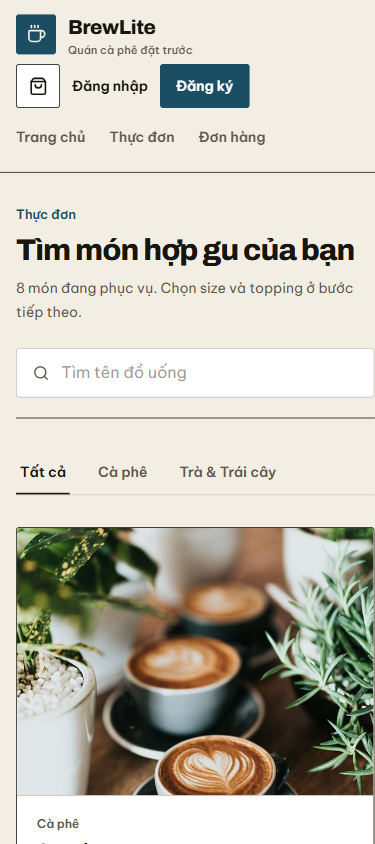
\includegraphics[width=0.26\textwidth]{../figures/as2/view/01-menu-mobile.png}
\caption{Màn hình menu mobile-first của MVP Sprint 1}
\label{figB:menu-s1}
\end{figure}

\begin{table}[H]
\centering\small
\caption{Kết quả kiểm thử MVP Sprint 1}
\label{tabB:s1-test}
\begin{tabularx}{\textwidth}{@{}l X l@{}}
\toprule
\textbf{Hạng mục} & \textbf{Nội dung} & \textbf{Kết quả} \\
\midrule
% TODO(B): products.test.cjs, menu-filter.test.mjs, build web/api
\bottomrule
\end{tabularx}
\end{table}

\subsection{Task 4.4 -- Continuous Integration}
% TODO(B): pipeline install -> lint -> unit test -> build; chạy trên push/PR vào main;
% PR đỏ không được merge. Nêu số lần chạy thực tế nếu lấy được từ GitHub Actions.
\begin{table}[H]
\centering\small
\caption{Các bước trong workflow \file{ci.yml}}
\label{tabB:ci}
\begin{tabularx}{\textwidth}{@{}c l X@{}}
\toprule
\textbf{Bước} & \textbf{Lệnh} & \textbf{Điều kiện đạt} \\
\midrule
% TODO(B)
\bottomrule
\end{tabularx}
\end{table}

\paragraph{Minh chứng.}
% TODO(B): chụp 2 ảnh GitHub Actions: 1 run xanh, 1 run đỏ bị chặn merge.
% Lưu vào docs/report/figures/ci-pass.png, ci-fail.png rồi bỏ comment.
% \begin{figure}[H]
% \centering
% 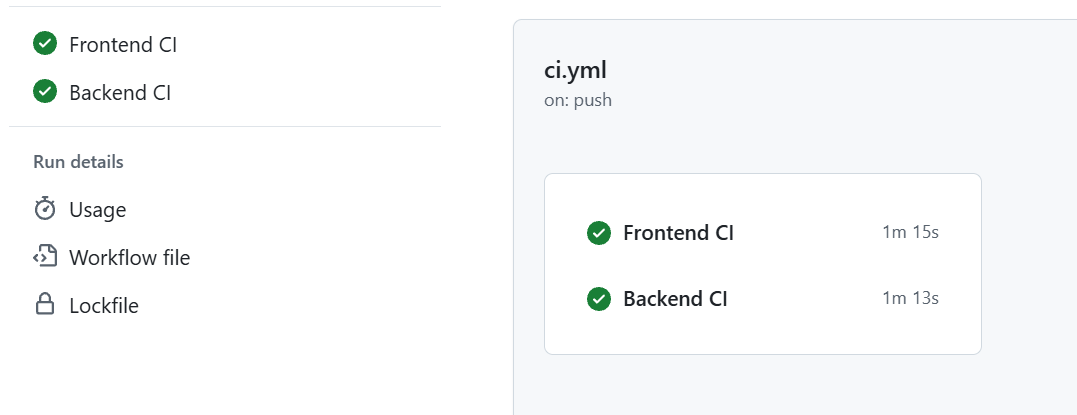
\includegraphics[width=0.9\textwidth]{figures/ci-pass.png}
% \caption{Pipeline CI thành công trên pull request}
% \label{figB:ci-pass}
% \end{figure}
